%%%%%%%%%%%%%%%%%%%%%%%%%%%%%%%%%%%%%%%%%%%%%%%%%%%%%%%%%%%%
%%%  Augmenting TV Newscasts via Entity Expansion  %%%
%%%%%%%%%%%%%%%%%%%%%%%%%%%%%%%%%%%%%%%%%%%%%%%%%%%%%%%%%%%%

\documentclass{llncs}

\newcommand{\superscript}[1]{\ensuremath{^{\textrm{#1}}}}

\usepackage{makeidx}  % allows for indexgeneration
\usepackage[hyphens]{url}
\usepackage{textcomp}
\usepackage{color}
\usepackage{listings}
\usepackage{multirow}
\usepackage{mathtools}
\usepackage{graphicx}
\usepackage{fancyvrb}
\usepackage{amsmath}
\usepackage{graphicx}
\usepackage[font=small,labelfont=bf]{caption}
\setcounter{MaxMatrixCols}{20}
\usepackage{pbox}
\usepackage{amsfonts}


% listing styles
\lstset{numbers=left, numberstyle=\tiny,basicstyle=\ttfamily\scriptsize, tabsize=2, keywordstyle=\underbar, stringstyle=\small, backgroundcolor=\color[gray]{0.94}, framexleftmargin=2pt}
\lstdefinestyle{rdfa}{numberblanklines=true, morekeywords={}}


\begin{document}
\frontmatter          % for the preliminaries
\pagestyle{headings}  % switches on printing of running heads
\mainmatter              % start of the contributions

\title{Exploring the Semantic Context of News Events}
\author{Jos\'e Luis Redondo Garc\'ia\inst{2}, Michiel Hildebrand\inst{1}, Lilia Perez Romero\inst{1}, Giuseppe Rizzo\inst{2}, Rapha\"el Troncy\inst{2}}
\institute{EURECOM, Sophia Antipolis, France, \\
\email{\{redondo, giuseppe.rizzo, raphael.troncy\}@eurecom.fr}
\and
CWI, Amsterdam, The Netherlands, \\
\email{\{M.Hildebrand, L.Perez\}@cwi.nl}
}


\maketitle              % typeset the title of the contribution

%%%%%%%%%%%%%%%%%%
%%%  Abstract  %%%
%%%%%%%%%%%%%%%%%%

\begin{abstract}

Relying on subtitles of an audiovisual content to extract named entities is a common method for describing and annotating news and events. However, previous studies on this area [Lilia] have revealed that this approach has multiple limitations, and what is being explicitly said in a particular news document is insufficient for reconstructing the whole context of the event. 

In this paper we demonstrate that by leveraging in Semantic Web techniques and the power of non-structured documents we can --automatically-- generate a description of the event that is much closer to the vision that the humans have about it. The result of this approach is not a simple set of entities, but a ranked list of concepts wich can be used to be displayed on a device o derive further enrichments.

We have evaluated the approach by comparing our automatic generated context with the one expected by the viewers over a set of newscasts from the BBC.

\keywords{Semantic Video Annotation, Media Fragments, Summarization}
\end{abstract}

%%%%%%%%%%%%%%%%%%%%%%%%%
%%%  1. Introduction  %%%
%%%%%%%%%%%%%%%%%%%%%%%%%

\section{Introduction}
The set of entities obtained from a traditional named entity extraction operation is normally insufficient and incomplete for expressing the context of a news event. Sometimes, some entities spotted over a particular document are not disambiguated because the textual clues surrounding the entity are not precise enough for the name entity extractor, while in other cases, they are simply not mentioned in the transcripts while being relevant for understanding the story. This is an inherent problem in information retrieval tasks: a single description about the same resource does not necessarily summarize the whole picture.

The named entity expansion operation relies on the idea of retrieving and analyzing additional documents from the Web where the same event is also described. By increasing the size of set of documents to analyse, we increase the completeness of the context and the representativeness of the list of entities, reinforcing relevant entities and finding new ones that are potentially interesting inside the context of that news item.

* Demo in ESWC, paper in SNOW

* Comments on Lilia's paper (maybe include some figures here?)

* State of the art in News applications and supporting tools for journalist.

% State of the Art on Semantic annotation
* State of the Art on Semantic annotation.
Concerning the multimedia annotation the literature covers a wide range of different analysis techniques~\cite{ballan2011event}. One of the main approaches consists on running Named Entity Recognition (NER) over the textual information attached to particular video fragment. Those techniques are an essential component within the Information Extraction field that focus on: identifying atomic information units in texts, named entities; classifying entities into predefined categories (also called context types) and linking to real world objects using web identifiers (Named Entity Disambiguation). A growing number of APIs provide such a service, like AlchemyAPI\footnote{\fontsize{8pt}{1em}\selectfont \url{http://www.alchemyapi.com/}} or DBpedia Spotlight\footnote{\fontsize{8pt}{1em}\selectfont \url{http://spotlight.dbpedia.org/}}. If the textual information attached to a video contains temporal references (e.g. subtitles), it is possible to align the entities with the time when they appear in the video. In this line, Yunjia et al.~\cite{yunjia2013} have probed that named entity recognition techniques applied on video subtitles can produce good results for video classification. 

%%%%%%%%%%%%%%%%%%%%%%%%%%%%%%%%%%
%%%  News Concept Expansion Algorithm    %%%
%%%%%%%%%%%%%%%%%%%%%%%%%%%%%%%%%%
\section{Generating and Displaying Hot Spots in Web Videos}
\label{sec:ConceptExpansion}

\subsection{Query Generation}
The \emph{Five W's} is a popular concept of information gathering in journalistic reporting. It captures the main aspects of a story: who, when, what, where, and why~\cite{LiJia2007}. We try to represent the news item in terms of four of those five W's (who is involved in the event, where the event is taking place, what the event is about, and when it has happened) in order to generate a query that retrieves documents associated to the same event.

First, the original entities are mapped to the NERD Core ontology, which considers 10 main classes: Thing, Amount, Animal, Event, Function, Organization, Location, Person, Product and Time. From those ten different categories, we generalize to three classes: the Who from \url{nerd:Person} and \url{nerd:Organization}, the Where from \url{nerd:Location}, and the What from the rest of NERD types after discarding \url{nerd:Time} and \url{nerd:Amount}. The When or so-called temporal dimension does not need to be computed since it is considered to be provided by the video publisher.

After generating the three sets of entities, the next step consist in ranking them in relevance according to a weighted sum of two different dimensions: their frequency in the transcripts and their former relevance scores coming from the named entity extractors. We have defined the function \emph{filterEntities(S)} for selecting the $n$ entities inside the set of entities $S$ whose relative relevance

\begin{equation}
R_{rel}\left ( e_{i}, S \right ) = R\left ( e_{i} \right ) / Avg \left ( R\left ( e_{i} \right )  \right )
\end{equation}

falls into the upper quarter of the interval

\begin{equation}
\left [ max\left ( R_{rel}\left ( e_{i}, S \right )  \right ) -min\left (  R_{rel}\left ( e_{i}, S \right ) \right ) \right ]
\end{equation}

The final query is a pair

\begin{equation}
\text{Query}_{Event} =\left [ \text{textQuery}, t \right ]
\end{equation}

where \textit{textQuery} is the result of concatenating the labels of the most relevant entities in the sets Who, What, Where in that particular order, and $t$ the time period dimension. This query generation is depicted in the upper part of Figure~\ref{fig:namedEntityExpansion}.

\subsection{Document Retrieval}
Once $\text{Query}_{Event}$ is built out of the original set of named entities, it will be ready to be injected into a document search engine where additional descriptions about the news event can be found. In this situation, the kind of query generated in the previous step and the search engine chosen should be closely tied in order to maximize the quality of the obtained results. The different behavior of search engines make some alternatives more suitable than others for certain kinds of events. The way the resulting documents change in the search engines for a particular kind of event is a research question that will not be studied in this paper.

In this paper, we rely on the Google Search REST API service\footnote{\fontsize{8pt}{1em}\selectfont  \url{http://ajax.googleapis.com/ajax/services/search/web?v=1.0}} by launching a query with the text \textit{textQuery}. Due to quota restrictions imposed by Google, the maximum number of retrieved document is set to 30. However, as shown in the evaluation described in the Section~\ref{sec:evaluation}, this is enough for significantly extending the initial set of entities directly spotted by NERD.

Concerning the temporal dimension, we only keep the documents published in the time period $t+t_{e}$. We increase the original event period in $t_{e}$ because documents concerning a news event are not always published during the time of the action is taking place but some hours or days after. The value of $t_{e}$ depends on many factors such as the nature of the event itself (whether it is a brief appearance in a media, or part of a longer story with more repercussion) or the kind of documents the search engine is indexing (from very deep and elaborated documents that need time to be published, to short post quickly generated by users). Based on the simple assumption that that the longer is an event, and the longer it is likely to generate buzzes, we approximated  $t_{e} = t$ which means that we also consider document published during the course of an event.

The middle part of Figure~\ref{fig:namedEntityExpansion} shows this process. The query is input in the search engine in order to retrieve other documents that report on the same event discussed in the original video. Those documents (colored in black in the Figure~\ref{fig:namedEntityExpansion}) will be further processed to increase the size of the collection and get additional insights about the news item.

\begin{figure}[h!]
\centering
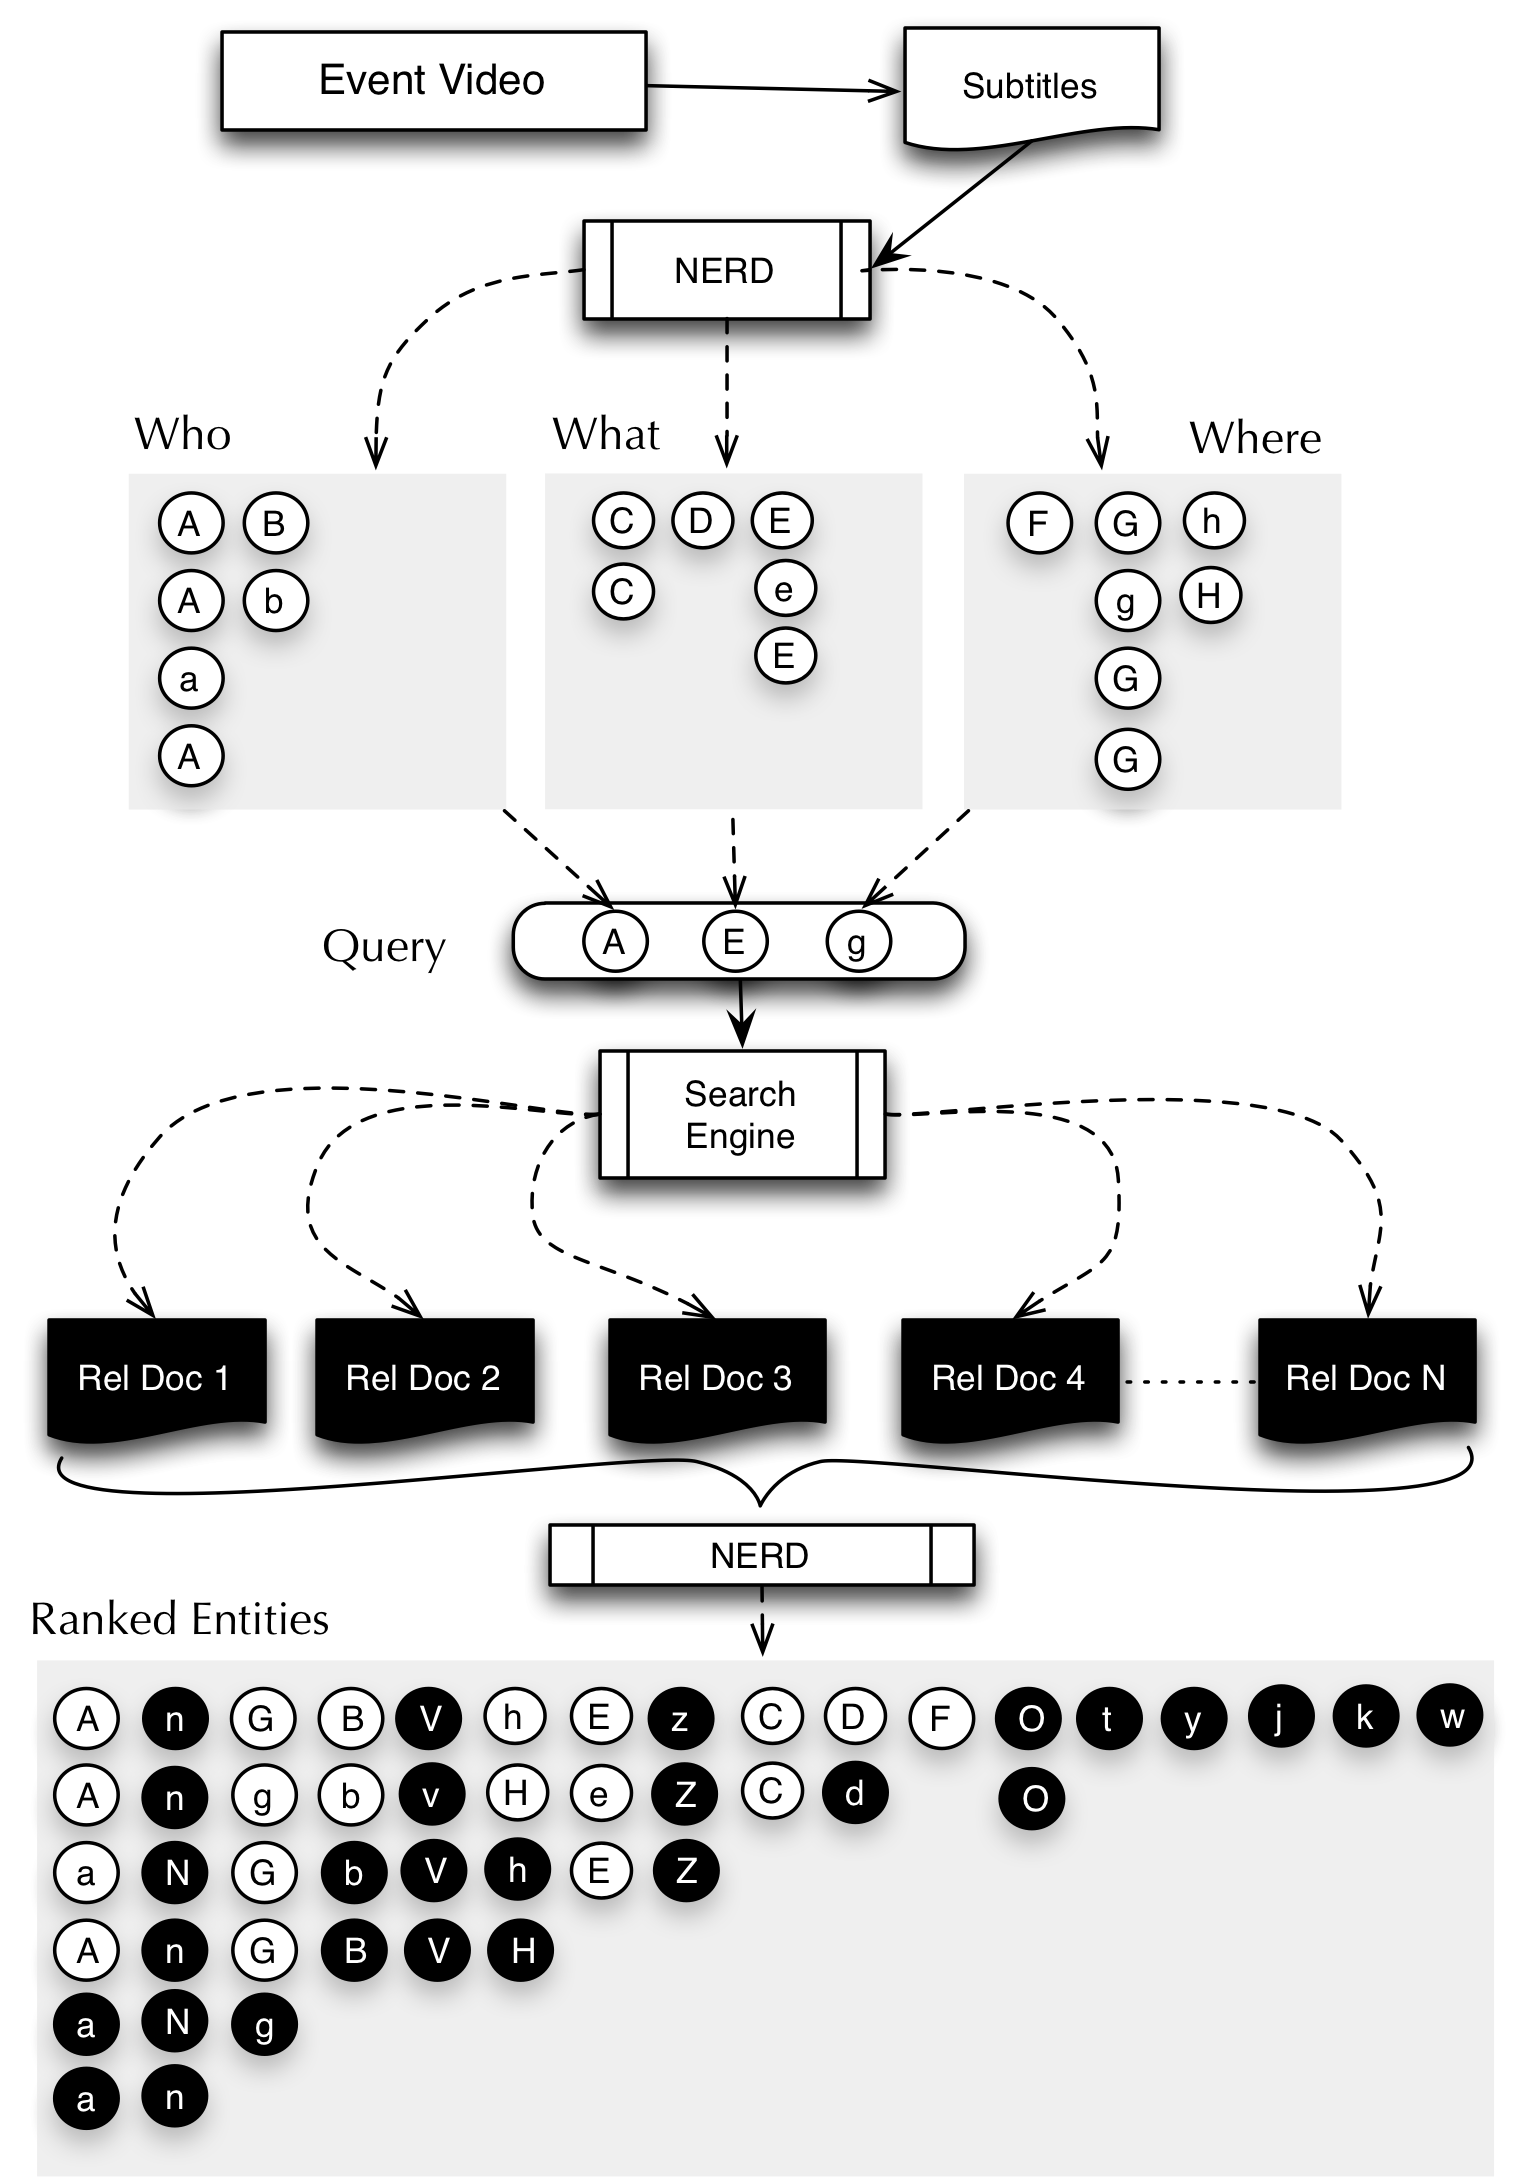
\includegraphics[width=0.5\textwidth]{figure/ExpansionDiagram}
\caption{Schema of Named Entity Expansion Algorithm.}
\label{fig:namedEntityExpansion}%\end{figure}
\end{figure}

\subsection{Entity Clustering}
In this phase, the additional documents which have just been retrieved are now processed and analyzed in order to extend and re-rank the original set of entities and consequently get a better insight about the event. Since most of the resources retrieved are Web pages, HTML tags and other annotations are removed, keeping only the main textual information. This plain text is then analyzed by the NERD framework in order to extract more named entities.

In order to calculate the frequency of a particular resource within the entire corpora, we group the different appearances of the same instance and check their cardinality. This is not a trivial task since the same entity can appear under different text labels, contain typos or have different disambiguation URL's pointing to the same resource. We performed a centroid-based clustering operation over the instances of the entities. We considered the centroid of a cluster as the entity with the most frequent disambiguation URL's that also have the most repeated labels. As distance metric for comparing pairs of entities, we applied strict string similarity over the URL's, and in case of mismatch, the Jaro-Winkler string distance~\cite{winkler2006overview} over the labels. The output of this phase is a list of clusters containing different instances of the same entity.

\subsection{Results}
Non ranked list of concepts at the end of this phase.

%%%%%%%%%%%%%%%%%%%%%%%%%%%%%%%%%%
%%%  Ranking and Filtering Concepts from Expansion   %%%
%%%%%%%%%%%%%%%%%%%%%%%%%%%%%%%%%%
\section{Ranking and Filtering Concepts from Expansion}
\label{sec:Ranking}

The unordered set of entities has to be ranked for (1) propose prominent concepts to the viewer (2) get rid of the long queue of entities and noise produced by during the expansion process.

\subsection{Frequency-based Ranking}

\subsection{TF-IDF  Ranking}

\subsection{Ranking based on Popularity}

\subsection{Ranking based DBpedia clues}
(Presented in SNOW 2014)

\subsection{Rules based re-ranking}
Based in the conclusions from Lilia's report. In her study, Lilia has indicated how certain NERD types are preferred by users:
- Most of the Organizations were interesting (figures in Excel file)
- Persons 
- Normally less interested in Places and other NERD categories.

\subsection{Deciding on the Best Ranking Approach}
\label{sec:decidingRanking}
Introduce Lilia's dataset, 5 videos, expert involved. We are going to use this dataset for selecting wich is the most appropriate ranking algorithm

%%%%%%%%%%%%%%%%%%%%%%%
%%%  4. EVALUATION  %%%
%%%%%%%%%%%%%%%%%%%%%%%

\section{Evaluation}
\label{sec:Evaluation}

\subsection{Dataset for evaluation}
Building the ground truth. Survey on 15 videos from the BBC about international facts. Evaluated over people in different countries.

* Explain the form: show automatically generated concepts + empty fields for suggesting possible missing entities.

* Show the results of the survey.

\subsection{Effectiveness of the approach}
 
Measurements in terms of Recall and Precision, at 7 (average number of results selected as relevant by the users)
 (No hay relaci�n directa entre el numero de entidades seleccionadas. Se coge por tanto la media.)
 
In the evaluation we will focus in the highly ranked relevant documents. Similar to Web search engines, we will apply an evaluation measure which will try to find as many relevant documents as possible, while still keeping the  premise that the top ranked documents are the most important. We will not perform measures in terms of efficiency. Even this kind of study is easier to quantify (most of the time it can be measured automatically with a timer instead of with costly relevance judgments) this falls outside the scope of this paper. 

Those are the key efficiency measurements we would like to perform (Question: Should we try to do the same in Section "Selecting Ranking Pp"):

** Mean average precision at 10  - single number summary, popular measure, pooled
relevance judgments.

** Average NDCG - single number summary for each rank level, emphasizes top ranked documents, relevance judgments only needed to a speciffc rank depth
(in our example 10).

** Recall-precision graph - conveys more information than a single number measure, pooled relevance judgments.

** Average precision at rank 10 - emphasizes top ranked documents, easy to understand, relevance judgments limited to top 10.

We will use the same same ranking algorithm on five different queries. We aim of an averaging technique is to summarize the effectiveness of a specific ranking algorithm across a collection of queries. Different queries will then have different numbers of relevant documents, as is the case in this example. Figure about recall-precision for the top ten rank positions.

%%%%%%%%%%%%%%%%%%%%%%%
%%%  4. Conclusions  %%%
%%%%%%%%%%%%%%%%%%%%%%%

\section{Conclusions}
\label{sec:conclusions}

We presented an approach for context-aware annotating news events, designed to precisely harvest program descriptions starting from named entities recognized in TV video transcripts. Because the entities initially spotted are typically insufficient for covering the broader range of concepts that best describe a particular news clip, we expanded this set by analyzing additional textual documents about the same event.

The evaluation indicates that we can successfully expand the initial set of recognized entities with more relevant concepts not detected by pure named entity recognition approaches and produce a more accurate ranking of important concepts that brings forward entities which user are more interested about.

Future: tailor ranking to particular types of news: sport, politics, regional, international, opinion, etc.

%%%%%%%%%%%%%%%%%%%%%%%%%
%%%  Acknowledgments  %%%
%%%%%%%%%%%%%%%%%%%%%%%%%

\section*{Acknowledgments}
This work was partially supported by the European Union's 7th Framework Programme via the project LinkedTV (GA 287911).

%%%%%%%%%%%%%%%%%%%%%%
%%%  Bibliography  %%%
%%%%%%%%%%%%%%%%%%%%%%
\bibliographystyle{abbrv}
\bibliography{NewsConceptExpansion}

\end{document}
